%% bare_conf.tex
%% V1.4
%% 8/27/2019
%% by Dalton Cole
%%
\documentclass[conference]{IEEEtran}


% *** CITATION PACKAGES ***
\usepackage{cite}


% *** GRAPHICS RELATED PACKAGES ***
\usepackage[pdftex]{graphicx}
% declare the path(s) where your graphic files are
% \graphicspath{{../pdf/}{../jpeg/}}
% and their extensions so you won't have to specify these with
% every instance of \includegraphics
% \DeclareGraphicsExtensions{.pdf,.jpeg,.png}


% *** MATH PACKAGES ***
\usepackage[cmex10]{amsmath}

% *** SPECIALIZED LIST PACKAGES ***
\usepackage{algorithmic}

% *** ALIGNMENT PACKAGES ***
\usepackage{array}
% Frank Mittelbach's and David Carlisle's array.sty patches and improves
% the standard LaTeX2e array and tabular environments to provide better
% appearance and additional user controls. As the default LaTeX2e table
% generation code is lacking to the point of almost being broken with
% respect to the quality of the end results, all users are strongly
% advised to use an enhanced (at the very least that provided by array.sty)
% set of table tools. array.sty is already installed on most systems. The
% latest version and documentation can be obtained at:
% http://www.ctan.org/tex-archive/macros/latex/required/tools/

% *** SUBFIGURE PACKAGES ***
\ifCLASSOPTIONcompsoc
  \usepackage[caption=false,font=normalsize,labelfont=sf,textfont=sf]{subfig}
\else
  \usepackage[caption=false,font=footnotesize]{subfig}
\fi

% *** FLOAT PACKAGES ***
\usepackage{fixltx2e}

% *** PDF, URL AND HYPERLINK PACKAGES ***
\usepackage{url}
% Basically, \url{my_url_here}.

% correct bad hyphenation here
\hyphenation{op-tical net-works semi-conduc-tor}


%%%%%%%%%%%%%%%%%%%%%%%%%%%%%%%%%%%%%%%%%%%%%%%%%%%%%%%%%%%%%%%%%%%%%%%%%%%%%%%%%%%%%%%%%%%%%%%%%%%
\begin{document}
%
% paper title
% can use linebreaks \\ within to get better formatting as desired
% Do not put math or special symbols in the title.
\title{TODO}


% author names and affiliations
% use a multiple column layout for up to three different
% affiliations
\author{
\IEEEauthorblockN{Dalton Cole}
\IEEEauthorblockA{Department of Computer Science\\
Missouri University of Science and Technology\\
Rolla, Missouri 65409-0350, USA\\
Email: drcgy5@mst.edu}
\and
\IEEEauthorblockN{Bruce McMillin}
\IEEEauthorblockA{Department of Computer Science\\
Missouri University of Science and Technology\\
Rolla, Missouri 65409-0350, USA\\
Email: ff@mst.edu}}

% make the title area
\maketitle

% As a general rule, do not put math, special symbols or citations
% in the abstract
\begin{abstract}
The abstract goes here.
\end{abstract}

% no keywords

% For peer review papers, you can put extra information on the cover
% page as needed:
% \ifCLASSOPTIONpeerreview
% \begin{center} \bfseries EDICS Category: 3-BBND \end{center}
% \fi
%
% For peerreview papers, this IEEEtran command inserts a page break and
% creates the second title. It will be ignored for other modes.
\IEEEpeerreviewmaketitle



\section{Introduction}
% no \IEEEPARstart
Intro

%\hfill mds 
%\hfill December 27, 2012

% Sub and subsub section EXAMPLE
%\subsection{Subsection Heading Here}
%Subsection text here.

%\subsubsection{Subsubsection Heading Here}
%Subsubsection text here.

%%%%%%%%%%%%%%%%%%%%%%%%%%%%%%%%%%%%%%%%%%%%%%%%%%
\section{Methodology}

An overview of the system is outlined in Figure \ref{fig:system_overview}. The following subsections outline in detail how each partition of the system functions. For how data was collected, see Section \ref{Experimental Evaluation}.

\begin{figure}[h!]
  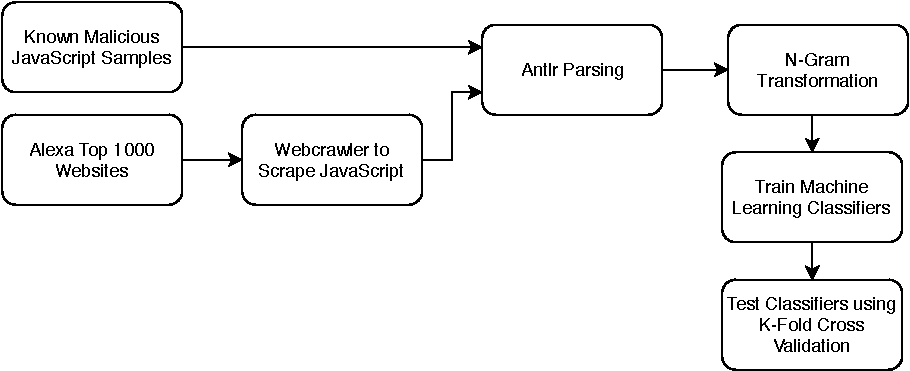
\includegraphics[scale=0.5]{figures/grammar_malware_overview.pdf}
  \caption{System Overview}
  \label{fig:system_overview}
\end{figure}


% Overview - Mention overview table

\subsection{Antlr}

Antlr was used to parse the grammar \cite{antlr}. Antler is a framework designed to automatically generate code in a number of languages. The resulting supplementary files can be used to tokenize and parse given inputs. Antlr requires tokens and grammatical rules to be defined for the desired language in a g4 file. Antlr is designed for context-free grammars (CFG), however, by adding additional logic that is programming language specific, Antlr can handle context-sensitive languages.

Antlr parses samples using a LL(*) parser, which is a top-down approach. Top-down approaches work by starting at the top level of a parse tree and matches as it traverses down the tree. LL(*) performs leftmost deviation as it reads in tokens from left to right. The amount of tokens read in at a time to determine which grammar rule to use is determined by the * value. If $* = 1$, then only one token is required at a time to know which grammar rule to expand next.


\subsection{N-Gram}

A list of grammatical rules in order of which they were parsed is extracted from a given sample using Antlr. These rules were then grouped in over-lapping sequences of n rules where each sequence differed by its neighboring sequences by one rule. These sequences are called n-grams. A snippet of a n-gram extracted from our system can be found in Figure \ref{fig:n-gram-example}. Due to memory limitations, only sequences where $n = \{1, 2, 3\}$ were explored. To generate a feature vector of set length, every possible n-gram was composed.

\begin{figure}[h!]
\centering
  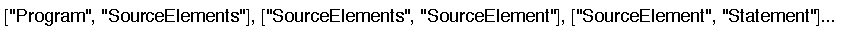
\includegraphics[scale=0.5]{figures/n_gram_example.pdf}
  \caption{N-Gram Example where N = 2}
  \label{fig:n-gram-example}
\end{figure}


% Explain why a different number of features were used
% For memory and accuracy testing, we used a different
%   number of features for different tests

\subsection{Feature Reduction} \label{Methodology - Feature Reduction}

Due to the large number of features that n-gram produces, feature reduction is required to reduce the memory usage to a usable level. In order to read in saved data, incremental principal component analysis (IPCA) was selected. IPCA is able to read in information from disk in batches. From each read, IPCA finds orthogonal eigen vectors. After all rows of the dataframe have been read in, the top n eigen vectors with the most variance are selected to represent the features of the data. When the number of features are less than n, feature reduction is not applied. %This occurs in the trimmed and extra trimmed 1-gram datasets.

\subsection{Machine Learning}

A number of different machine learning methods were employed. These methods were chosen so the results could be compared to TODO LIST REFERENCES. K-Fold cross validation was used to train and test each machine learning classifier.

\subsubsection{Decision Trees}

entropy

\subsubsection{Random Forests}

\subsubsection{Neural Network}

\subsubsection{Naive Bayes}

\subsubsection{Gradient Decent}

\subsubsection{K-Nearest-Neighbors}

%%%%%%%%%%%%%%%%%%%%%%%%%%%%%%%%%%%%%%%%%%%%%%%%%%
\section{Experimental Evaluation} \label{Experimental Evaluation}

% Mention that JavaScript was used and why

\subsection{Benign Data Collection}

The benign data set consisted of JavaScript samples scraped from the top 1000 Alexa websites \cite{alexa}. Due to these site's popularity, it was assumed that each javascript sample scrapped from these sites were benign.

The python library scrapy was used to create a web-crawler and scrapper \cite{scrapy}. A set of starting URLs and acceptable domains were given to scrapy that consisted of the top 1000 Alexa websites. From here, any javascript that was enclosed in HTML script tags were scrapped from the site and saved into a hash-table. A hash-table was used to guarantee unique samples. A total of 201,901 scripts were scrapped using this method. Due to our use of Antlr, malformed JavaScript samples could not be parsed. The main malformation that was not accepted was the lack of use of semicolons. If a script did not use semicolons to end statements, the script was considered malformed and discarded. A full list of what is considered malformed can be found at \cite{javascript_grammar}. After malformed samples were removed from the set of possible scripts, 140,437 scripts remained. These scripts were feed into Antlr using the JavaScript grammar defined in \cite{javascript_grammar}. From Antlr the order in which the grammatical rules were parsed in were returned.

\subsection{Malicious Data Collection}

Malicious data consisted of known malicious JavaScript samples obtained from \cite{malicious_javascript_repo}. The majority of this malware was collected between 2015 and 2017. A random sample was ran through VirusTotal in order to verify that leading anti-virus scanners recognized the samples as malicious \cite{virustotal}. All samples that were randomly selected was marked malicious by VirusTotal. A total of 39,471 JavaScript samples were obtained. Similarly to the benign samples collected, some scripts were malformed. After removing the malformed samples, 15,096 samples remained. Using Antlr, the order in which the grammatical rules were parsed in were returned.

\subsection{Feature Reduction}

% Explain why feature Reduction was/was not used
Due to the large number of features that n-gram produces, three different feature sets were used. An unabridged dataset containing 112 features. This unabridged dataset contains every grammatical non-terminal in the original JavaScript grammar used to parse the language. From this unabridged dataset, two additional datasets were generated. A trimmed dataset containing 62 rules were generated by combining every Expression grammatical rule into a single grammatical rule. By combining similar rules into a single rule, it is hoped that not much information is lost. A third extra trimmed dataset was constructed by further combining similar rules until only 40 features remained.

The reason this feature reduction was required is due to n-gram's exponential nature. When using 1-gram with the original dataset, only 112 features are needed. However, when using 2-gram, 12544 features are required. With this exponential growth, more memory is required to store those features. In addition, a very sparse matrix will be produced since most of the n-gram rules will not be seen in the source program.

In addition to the above feature reduction methods, incremental principal component analysis (IPCA) was employed to further reduce the features. A brief overview of how IPCA functions is reviewed in Section \ref{Methodology - Feature Reduction}. One hundred orthogonal vectors with the most variance was selected. One hundred features were selected because it gave a good compromise to the number of features in the 1-gram unabridged dataset. With the number of samples explored, 100 features will easily fit into memory without the need to save to disk, thus training times were greatly reduced.

\subsection{Classifier Training}

% Used equal number of benign and malicious samples
For classification training, an equal number of benign and malicious samples were selected from each dataset. Given the size of the malicious dataset, 15,000 samples from each classification was used to train the models. Choosing an equal number of samples in each class was decided upon due to two reasons. 

Firstly, the imbalanced class issues for the majority of machine learning methods used in this paper have been explored in \cite{sun2009classification}. With regards to decision trees, Sun et al. described how during the pruning phase of generating a decision tree, the leaf nodes representing the minority class have a good chance of being pruned since they have little effect on the overall accuracy of that branch. In addition, with respect to neural networks, they found that the majority class in skewed data tends to dominate the gradient vector. The minority class may even need to traverse in an uphill direction to find the optimal values. 

Secondly, accuracy and precision are positively effected by skewed data. Generally, classifiers are able to classify the majority class correctly a larger percentage of the time. Strictly looking at accuracy, classifier accuracy will be inflated due to classifying the majority class correctly more often. This diminishes the actual results of the minority class that we are concerned about \cite{jeni2013facing}.

% Site paper saying skewed data increases accuracy


% over sampling. Reference a couple papers showing that undersampling is better than over sampling
% recall and precision are balanced


\subsection{Results}

Recall, Precision, and $F_1$ score are the three primary metrics used to compare each result. Formulas used to calculate these can be found in Equation \ref{equ:recall}, Equation \ref{equ:precision}, and Equation \ref{equ:f1_score}, respectively.

\begin{equation}
	Recall = \frac{True Positive}{True Positive + False Negative}
	\label{equ:recall}
\end{equation}

\begin{equation}
	Precision = \frac{True Positive}{True Positive + False Positive}
	\label{equ:precision}
\end{equation}

\begin{equation}
	F_1 = 2 * \frac{Precision * Recall}{Precision + Recall}
	\label{equ:f1_score}
\end{equation}

\subsubsection{Full Feature Set}

The results using the full unabridged original feature set can be found in Table \ref{table:full}. Only n-grams where $n = {1, 2}$ are explored due to memory limitations. The total number of features are 112 and 12544 for each respective n-gram. In general, each metric improved when more features were used. Decision tree, random forests, neural network, and the stochastic gradient decent classifier perform nearly equally and better than other algorithms with regards to their $F_1$ score.

\subsubsection{Full Feature Set with Feature Reduction}

The full unabridged original feature set with feature reduction can be found in Table \ref{table:full_feature_selectiond}. The 112 and 12544 features in the full feature set where $n = {1, 2}$ is reduced to 100 features. This is done through incremental principal component analysis (IPCA) which is described in Section \ref{Methodology - Feature Reduction}. Desicion tree, random forest, and stochastic gradient decent classifier performed better than other algorithms tested.

\subsubsection{Trimmed Feature Set}


% Lots of tables
\begin{center}
\begin{table*}[htbp]
\caption{Full Feature}
\label{table:full}
\resizebox{\textwidth}{!}{%
\renewcommand{\arraystretch}{1.3}
\begin{tabular}{| c | c | c | c | c | c | c | c | c | c |}
\hline
N-Gram	& Algorithm	& Total Features	& True Positive \%	& False Positive \%	& True Negative \%	& False Negative \%	& Recall	& Precision	& $F_1$ \\
\hline \hline
1 	& 	Decision Tree 	& 	112 	& 	98.7267 	& 	6.0 	& 	94.0 	& 	1.2733 	& 	0.9873 	& 	0.9427 	& 	0.9645 		 \\
\hline
1 	& 	Random Forest 	& 	112 	& 	98.72 	& 	5.88 	& 	94.12 	& 	1.28 	& 	0.9872 	& 	0.9438 	& 	0.965 		 \\
\hline
1 	& 	Neural Network 	& 	112 	& 	94.76 	& 	6.58 	& 	93.42 	& 	5.24 	& 	0.9476 	& 	0.9351 	& 	0.9413 		 \\
\hline
1 	& 	Naive Bayes 	& 	112 	& 	99.8333 	& 	76.9867 	& 	23.0133 	& 	0.1667 	& 	0.9983 	& 	0.5646 	& 	0.7213 		 \\
\hline
1 	& 	Stochastic Gradient Descent Classifier 	& 	112 	& 	98.08 	& 	7.16 	& 	92.84 	& 	1.92 	& 	0.9808 	& 	0.932 	& 	0.9558 		 \\
\hline
1 	& 	K-Nearest Neighbors 	& 	112 	& 	82.3933 	& 	0.1333 	& 	99.8667 	& 	17.6067 	& 	0.8239 	& 	0.9984 	& 	0.9028 		 \\
\hline
2 	& 	Decision Tree 	& 	12544 	& 	99.9667 	& 	5.44 	& 	94.56 	& 	0.0333 	& 	0.9997 	& 	0.9484 	& 	0.9734 		 \\
\hline
2 	& 	Random Forest 	& 	12544 	& 	99.9333 	& 	5.3333 	& 	94.6667 	& 	0.0667 	& 	0.9993 	& 	0.9493 	& 	0.9737 		 \\
\hline
2 	& 	Neural Network 	& 	12544 	& 	99.9933 	& 	5.42 	& 	94.58 	& 	0.0067 	& 	0.9999 	& 	0.9486 	& 	0.9736 		 \\
\hline
2 	& 	Naive Bayes 	& 	12544 	& 	99.96 	& 	31.7867 	& 	68.2133 	& 	0.04 	& 	0.9996 	& 	0.7587 	& 	0.8627 		 \\
\hline
2 	& 	Stochastic Gradient Descent Classifier 	& 	12544 	& 	99.96 	& 	5.52 	& 	94.48 	& 	0.04 	& 	0.9996 	& 	0.9477 	& 	0.9729 		 \\
\hline
2 	& 	K-Nearest Neighbors 	& 	12544 	& 	86.12 	& 	0.14 	& 	99.86 	& 	13.88 	& 	0.8612 	& 	0.9984 	& 	0.9247 		 \\
\hline
\end{tabular}}
\end{table*}
\end{center}
\begin{center}
\begin{table*}[htbp]
\caption{Full Feature - Feature Selection}
\label{table:full_feature_selectiond}
\resizebox{\textwidth}{!}{%
\renewcommand{\arraystretch}{1.3}
\begin{tabular}{| c | c | c | c | c | c | c | c | c | c |}
\hline
N-Gram	& Algorithm	& Total Features	& True Positive \%	& False Positive \%	& True Negative \%	& False Negative \%	& Recall	& Precision	& $F_1$ \\
\hline \hline
1 	& 	Decision Tree 	& 	100 	& 	98.6733 	& 	5.8333 	& 	94.1667 	& 	1.3267 	& 	0.9867 	& 	0.9442 	& 	0.965 		 \\
\hline
1 	& 	Random Forest 	& 	100 	& 	98.64 	& 	5.6 	& 	94.4 	& 	1.36 	& 	0.9864 	& 	0.9463 	& 	0.9659 		 \\
\hline
1 	& 	Neural Network 	& 	100 	& 	95.7 	& 	61.9667 	& 	38.0333 	& 	4.3 	& 	0.957 	& 	0.607 	& 	0.7428 		 \\
\hline
1 	& 	Naive Bayes 	& 	100 	& 	95.7067 	& 	73.5067 	& 	26.4933 	& 	4.2933 	& 	0.9571 	& 	0.5656 	& 	0.711 		 \\
\hline
1 	& 	Stochastic Gradient Descent Classifier 	& 	100 	& 	98.36 	& 	7.0 	& 	93.0 	& 	1.64 	& 	0.9836 	& 	0.9336 	& 	0.9579 		 \\
\hline
1 	& 	K-Nearest Neighbors 	& 	100 	& 	84.7333 	& 	1.1733 	& 	98.8267 	& 	15.2667 	& 	0.8473 	& 	0.9863 	& 	0.9116 		 \\
\hline
2 	& 	Decision Tree 	& 	100 	& 	99.8867 	& 	5.58 	& 	94.42 	& 	0.1133 	& 	0.9989 	& 	0.9471 	& 	0.9723 		 \\
\hline
2 	& 	Random Forest 	& 	100 	& 	99.8133 	& 	5.3733 	& 	94.6267 	& 	0.1867 	& 	0.9981 	& 	0.9489 	& 	0.9729 		 \\
\hline
2 	& 	Neural Network 	& 	100 	& 	94.7867 	& 	34.2067 	& 	65.7933 	& 	5.2133 	& 	0.9479 	& 	0.7348 	& 	0.8279 		 \\
\hline
2 	& 	Naive Bayes 	& 	100 	& 	95.2667 	& 	40.7533 	& 	59.2467 	& 	4.7333 	& 	0.9527 	& 	0.7004 	& 	0.8073 		 \\
\hline
2 	& 	Stochastic Gradient Descent Classifier 	& 	100 	& 	99.9533 	& 	5.62 	& 	94.38 	& 	0.0467 	& 	0.9995 	& 	0.9468 	& 	0.9724 		 \\
\hline
2 	& 	K-Nearest Neighbors 	& 	100 	& 	92.7 	& 	2.64 	& 	97.36 	& 	7.3 	& 	0.927 	& 	0.9723 	& 	0.9491 		 \\
\hline
\end{tabular}}
\end{table*}
\end{center}
\begin{center}
\begin{table*}[htbp]
\caption{Trimmed Features}
\label{table:trimmed}
\resizebox{\textwidth}{!}{%
\renewcommand{\arraystretch}{1.3}
\begin{tabular}{| c | c | c | c | c | c | c | c | c | c |}
\hline
N-Gram	& Algorithm	& Total Features	& True Positive \%	& False Positive \%	& True Negative \%	& False Negative \%	& Recall	& Precision	& $F_1$ \\
\hline \hline
1 	& 	Decision Tree 	& 	62 	& 	99.92 	& 	10.34 	& 	89.66 	& 	0.08 	& 	0.9992 	& 	0.9062 	& 	0.9504 		 \\
\hline
1 	& 	Random Forest 	& 	62 	& 	99.92 	& 	10.2267 	& 	89.7733 	& 	0.08 	& 	0.9992 	& 	0.9072 	& 	0.951 		 \\
\hline
1 	& 	Neural Network 	& 	62 	& 	49.4 	& 	50.6 	& 	49.4 	& 	50.6 	& 	0.494 	& 	0.494 	& 	0.494 		 \\
\hline
1 	& 	Naive Bayes 	& 	62 	& 	100.0 	& 	98.4733 	& 	1.5267 	& 	0.0 	& 	1.0 	& 	0.5038 	& 	0.6701 		 \\
\hline
1 	& 	Stochastic Gradient Descent Classifier 	& 	62 	& 	98.4867 	& 	13.8867 	& 	86.1133 	& 	1.5133 	& 	0.9849 	& 	0.8764 	& 	0.9275 		 \\
\hline
1 	& 	K-Nearest Neighbors 	& 	62 	& 	65.4467 	& 	1.1933 	& 	98.8067 	& 	34.5533 	& 	0.6545 	& 	0.9821 	& 	0.7855 		 \\
\hline
2 	& 	Decision Tree 	& 	3844 	& 	99.9067 	& 	5.26 	& 	94.74 	& 	0.0933 	& 	0.9991 	& 	0.95 	& 	0.9739 		 \\
\hline
2 	& 	Random Forest 	& 	3844 	& 	99.8933 	& 	5.1933 	& 	94.8067 	& 	0.1067 	& 	0.9989 	& 	0.9506 	& 	0.9742 		 \\
\hline
2 	& 	Neural Network 	& 	3844 	& 	13.9067 	& 	5.16 	& 	94.84 	& 	86.0933 	& 	0.1391 	& 	0.7294 	& 	0.2336 		 \\
\hline
2 	& 	Naive Bayes 	& 	3844 	& 	99.8533 	& 	49.1333 	& 	50.8667 	& 	0.1467 	& 	0.9985 	& 	0.6702 	& 	0.8021 		 \\
\hline
2 	& 	Stochastic Gradient Descent Classifier 	& 	3844 	& 	99.8933 	& 	6.1333 	& 	93.8667 	& 	0.1067 	& 	0.9989 	& 	0.9422 	& 	0.9697 		 \\
\hline
2 	& 	K-Nearest Neighbors 	& 	3844 	& 	86.04 	& 	0.06 	& 	99.94 	& 	13.96 	& 	0.8604 	& 	0.9993 	& 	0.9247 		 \\
\hline
\end{tabular}}
\end{table*}
\end{center}

\begin{center}
\begin{table*}[htbp]
\caption{Trimmed Features - Feature Selection}
\label{table:trimmed_feature_selected}
\resizebox{\textwidth}{!}{%
\renewcommand{\arraystretch}{1.3}
\begin{tabular}{| c | c | c | c | c | c | c | c | c | c |}
\hline
N-Gram	& Algorithm	& Total Features	& True Positive \%	& False Positive \%	& True Negative \%	& False Negative \%	& Recall	& Precision	& $F_1$ \\
\hline \hline
2 	& 	Decision Tree 	& 	100 	& 	99.84 	& 	5.4867 	& 	94.5133 	& 	0.16 	& 	0.9984 	& 	0.9479 	& 	0.9725 		 \\
\hline
2 	& 	Random Forest 	& 	100 	& 	99.7933 	& 	5.2667 	& 	94.7333 	& 	0.2067 	& 	0.9979 	& 	0.9499 	& 	0.9733 		 \\
\hline
2 	& 	Neural Network 	& 	100 	& 	98.3933 	& 	53.06 	& 	46.94 	& 	1.6067 	& 	0.9839 	& 	0.6497 	& 	0.7826 		 \\
\hline
2 	& 	Naive Bayes 	& 	100 	& 	94.4467 	& 	58.5467 	& 	41.4533 	& 	5.5533 	& 	0.9445 	& 	0.6173 	& 	0.7466 		 \\
\hline
2 	& 	Stochastic Gradient Descent Classifier 	& 	100 	& 	99.8667 	& 	6.14 	& 	93.86 	& 	0.1333 	& 	0.9987 	& 	0.9421 	& 	0.9695 		 \\
\hline
2 	& 	K-Nearest Neighbors 	& 	100 	& 	99.9533 	& 	5.4067 	& 	94.5933 	& 	0.0467 	& 	0.9995 	& 	0.9487 	& 	0.9734 		 \\
\hline
3 	& 	Decision Tree 	& 	100 	& 	99.8867 	& 	5.6867 	& 	94.3133 	& 	0.1133 	& 	0.9989 	& 	0.9461 	& 	0.9718 		 \\
\hline
3 	& 	Random Forest 	& 	100 	& 	99.7467 	& 	5.4667 	& 	94.5333 	& 	0.2533 	& 	0.9975 	& 	0.948 	& 	0.9721 		 \\
\hline
3 	& 	Neural Network 	& 	100 	& 	97.14 	& 	68.58 	& 	31.42 	& 	2.86 	& 	0.9714 	& 	0.5862 	& 	0.7311 		 \\
\hline
3 	& 	Naive Bayes 	& 	100 	& 	94.2 	& 	41.24 	& 	58.76 	& 	5.8 	& 	0.942 	& 	0.6955 	& 	0.8002 		 \\
\hline
3 	& 	Stochastic Gradient Descent Classifier 	& 	100 	& 	99.9267 	& 	5.86 	& 	94.14 	& 	0.0733 	& 	0.9993 	& 	0.9446 	& 	0.9712 		 \\
\hline
3 	& 	K-Nearest Neighbors 	& 	100 	& 	99.9667 	& 	5.56 	& 	94.44 	& 	0.0333 	& 	0.9997 	& 	0.9473 	& 	0.9728 		 \\
\hline
\end{tabular}}
\end{table*}
\end{center}

\begin{center}
\begin{table*}[htbp]
\caption{Extra Trimmed Features}
\label{table:extra_trimmed}
\resizebox{\textwidth}{!}{%
\renewcommand{\arraystretch}{1.3}
\begin{tabular}{| c | c | c | c | c | c | c | c | c | c |}
\hline
N-Gram	& Algorithm	& Total Features	& True Positive \%	& False Positive \%	& True Negative \%	& False Negative \%	& Recall	& Precision	& $F_1$ \\
\hline \hline
1 	& 	Decision Tree 	& 	40 	& 	95.6333 	& 	8.3733 	& 	91.6267 	& 	4.3667 	& 	0.9563 	& 	0.9195 	& 	0.9376 		 \\
\hline
1 	& 	Random Forest 	& 	40 	& 	95.6533 	& 	8.3 	& 	91.7 	& 	4.3467 	& 	0.9565 	& 	0.9202 	& 	0.938 		 \\
\hline
1 	& 	Neural Network 	& 	40 	& 	96.0867 	& 	11.6267 	& 	88.3733 	& 	3.9133 	& 	0.9609 	& 	0.8921 	& 	0.9252 		 \\
\hline
1 	& 	Naive Bayes 	& 	40 	& 	100.0 	& 	98.5867 	& 	1.4133 	& 	0.0 	& 	1.0 	& 	0.5036 	& 	0.6698 		 \\
\hline
1 	& 	Stochastic Gradient Descent Classifier 	& 	40 	& 	94.8867 	& 	12.8267 	& 	87.1733 	& 	5.1133 	& 	0.9489 	& 	0.8809 	& 	0.9136 		 \\
\hline
1 	& 	K-Nearest Neighbors 	& 	40 	& 	44.4133 	& 	0.1333 	& 	99.8667 	& 	55.5867 	& 	0.4441 	& 	0.997 	& 	0.6145 		 \\
\hline
2 	& 	Decision Tree 	& 	1600 	& 	99.9 	& 	5.1667 	& 	94.8333 	& 	0.1 	& 	0.999 	& 	0.9508 	& 	0.9743 		 \\
\hline
2 	& 	Random Forest 	& 	1600 	& 	99.8933 	& 	4.9667 	& 	95.0333 	& 	0.1067 	& 	0.9989 	& 	0.9526 	& 	0.9752 		 \\
\hline
2 	& 	Neural Network 	& 	1600 	& 	83.4267 	& 	27.28 	& 	72.72 	& 	16.5733 	& 	0.8343 	& 	0.7536 	& 	0.7919 		 \\
\hline
2 	& 	Naive Bayes 	& 	1600 	& 	99.94 	& 	51.22 	& 	48.78 	& 	0.06 	& 	0.9994 	& 	0.6612 	& 	0.7958 		 \\
\hline
2 	& 	Stochastic Gradient Descent Classifier 	& 	1600 	& 	99.94 	& 	5.94 	& 	94.06 	& 	0.06 	& 	0.9994 	& 	0.9439 	& 	0.9709 		 \\
\hline
2 	& 	K-Nearest Neighbors 	& 	1600 	& 	86.0533 	& 	0.08 	& 	99.92 	& 	13.9467 	& 	0.8605 	& 	0.9991 	& 	0.9246 		 \\
\hline
3 	& 	Decision Tree 	& 	64000 	& 	99.9333 	& 	5.3 	& 	94.7 	& 	0.0667 	& 	0.9993 	& 	0.9496 	& 	0.9739 		 \\
\hline
3 	& 	Random Forest 	& 	64000 	& 	99.8867 	& 	5.16 	& 	94.84 	& 	0.1133 	& 	0.9989 	& 	0.9509 	& 	0.9743 		 \\
\hline
3 	& 	Neural Network 	& 	64000 	& 	49.0067 	& 	50.9933 	& 	49.0067 	& 	50.9933 	& 	0.4901 	& 	0.4901 	& 	0.4901 		 \\
\hline
3 	& 	Naive Bayes 	& 	64000 	& 	99.9133 	& 	43.3733 	& 	56.6267 	& 	0.0867 	& 	0.9991 	& 	0.6973 	& 	0.8214 		 \\
\hline
3 	& 	Stochastic Gradient Descent Classifier 	& 	64000 	& 	99.9533 	& 	5.66 	& 	94.34 	& 	0.0467 	& 	0.9995 	& 	0.9464 	& 	0.9722 		 \\
\hline
3 	& 	K-Nearest Neighbors 	& 	64000 	& 	86.0733 	& 	0.1067 	& 	99.8933 	& 	13.9267 	& 	0.8607 	& 	0.9988 	& 	0.9246 		 \\
\hline
\end{tabular}}
\end{table*}
\end{center}

begin{center}
\begin{table*}[htbp]
\caption{Extra Trimmed Features - Feature Selection}
\label{table:extra_trimmed_feature_selected}
\resizebox{\textwidth}{!}{%
\renewcommand{\arraystretch}{1.3}
\begin{tabular}{| c | c | c | c | c | c | c | c | c | c |}
\hline
N-Gram	& Algorithm	& Total Features	& True Positive \%	& False Positive \%	& True Negative \%	& False Negative \%	& Recall	& Precision	& $F_1$ \\
\hline \hline
2 	& 	Decision Tree 	& 	100 	& 	99.84 	& 	5.3533 	& 	94.6467 	& 	0.16 	& 	0.9984 	& 	0.9491 	& 	0.9731 		 \\
\hline
2 	& 	Random Forest 	& 	100 	& 	99.7733 	& 	5.0333 	& 	94.9667 	& 	0.2267 	& 	0.9977 	& 	0.952 	& 	0.9743 		 \\
\hline
2 	& 	Neural Network 	& 	100 	& 	97.3733 	& 	77.8733 	& 	22.1267 	& 	2.6267 	& 	0.9737 	& 	0.5556 	& 	0.7075 		 \\
\hline
2 	& 	Naive Bayes 	& 	100 	& 	95.4467 	& 	64.2133 	& 	35.7867 	& 	4.5533 	& 	0.9545 	& 	0.5978 	& 	0.7352 		 \\
\hline
2 	& 	Stochastic Gradient Descent Classifier 	& 	100 	& 	99.8933 	& 	6.0 	& 	94.0 	& 	0.1067 	& 	0.9989 	& 	0.9433 	& 	0.9703 		 \\
\hline
2 	& 	K-Nearest Neighbors 	& 	100 	& 	88.9133 	& 	1.0867 	& 	98.9133 	& 	11.0867 	& 	0.8891 	& 	0.9879 	& 	0.9359 		 \\
\hline
3 	& 	Decision Tree 	& 	100 	& 	99.8533 	& 	5.56 	& 	94.44 	& 	0.1467 	& 	0.9985 	& 	0.9473 	& 	0.9722 		 \\
\hline
3 	& 	Random Forest 	& 	100 	& 	99.68 	& 	5.24 	& 	94.76 	& 	0.32 	& 	0.9968 	& 	0.9501 	& 	0.9729 		 \\
\hline
3 	& 	Neural Network 	& 	100 	& 	84.26 	& 	35.4267 	& 	64.5733 	& 	15.74 	& 	0.8426 	& 	0.704 	& 	0.7671 		 \\
\hline
3 	& 	Naive Bayes 	& 	100 	& 	95.24 	& 	43.86 	& 	56.14 	& 	4.76 	& 	0.9524 	& 	0.6847 	& 	0.7967 		 \\
\hline
3 	& 	Stochastic Gradient Descent Classifier 	& 	100 	& 	99.9067 	& 	5.76 	& 	94.24 	& 	0.0933 	& 	0.9991 	& 	0.9455 	& 	0.9715 		 \\
\hline
3 	& 	K-Nearest Neighbors 	& 	100 	& 	90.3333 	& 	1.7533 	& 	98.2467 	& 	9.6667 	& 	0.9033 	& 	0.981 	& 	0.9405 		 \\
\hline
\end{tabular}}
\end{table*}
\end{center}




%%%%%%%%%%%%%%%%%%%%%%%%%%%%%%%%%%%%%%%%%%%%%%%%%%
\section{Discussion}

% This was in Reults, moved to here. Need to make sure contextually, it makes sense
When $n = 1$, the feature vector only consists of boolean values of whether or not the grammatical rule was used to parse a sample or not. When $n > 1$, how grammatical rules interact with one another starts to be explored. The improved results show that the way malware is structured is different than benign samples. This is further highlighted in different feature sets.

When feature reduction was used, results were similar to the non reduced feature set.

% Metntion how a higher percentage of malformed malicious scripts were encountered when compared to the number of malformed bening scripts


%%%%%%%%%%%%%%%%%%%%%%%%%%%%%%%%%%%%%%%%%%%%%%%%%%
\section{Related Work}


% An example of a floating figure using the graphicx package.
% Note that \label must occur AFTER (or within) \caption.
% For figures, \caption should occur after the \includegraphics.
% Note that IEEEtran v1.7 and later has special internal code that
% is designed to preserve the operation of \label within \caption
% even when the captionsoff option is in effect. However, because
% of issues like this, it may be the safest practice to put all your
% \label just after \caption rather than within \caption{}.
%
% Reminder: the "draftcls" or "draftclsnofoot", not "draft", class
% option should be used if it is desired that the figures are to be
% displayed while in draft mode.
%
%\begin{figure}[!t]
%\centering
%\includegraphics[width=2.5in]{myfigure}
% where an .eps filename suffix will be assumed under latex, 
% and a .pdf suffix will be assumed for pdflatex; or what has been declared
% via \DeclareGraphicsExtensions.
%\caption{Simulation Results.}
%\label{fig_sim}
%\end{figure}

% Note that IEEE typically puts floats only at the top, even when this
% results in a large percentage of a column being occupied by floats.


% An example of a double column floating figure using two subfigures.
% (The subfig.sty package must be loaded for this to work.)
% The subfigure \label commands are set within each subfloat command,
% and the \label for the overall figure must come after \caption.
% \hfil is used as a separator to get equal spacing.
% Watch out that the combined width of all the subfigures on a 
% line do not exceed the text width or a line break will occur.
%
%\begin{figure*}[!t]
%\centering
%\subfloat[Case I]{\includegraphics[width=2.5in]{box}%
%\label{fig_first_case}}
%\hfil
%\subfloat[Case II]{\includegraphics[width=2.5in]{box}%
%\label{fig_second_case}}
%\caption{Simulation results.}
%\label{fig_sim}
%\end{figure*}
%
% Note that often IEEE papers with subfigures do not employ subfigure
% captions (using the optional argument to \subfloat[]), but instead will
% reference/describe all of them (a), (b), etc., within the main caption.


% An example of a floating table. Note that, for IEEE style tables, the 
% \caption command should come BEFORE the table. Table text will default to
% \footnotesize as IEEE normally uses this smaller font for tables.
% The \label must come after \caption as always.
%
%\begin{table}[!t]
%% increase table row spacing, adjust to taste
%\renewcommand{\arraystretch}{1.3}
% if using array.sty, it might be a good idea to tweak the value of
% \extrarowheight as needed to properly center the text within the cells
%\caption{An Example of a Table}
%\label{table_example}
%\centering
%% Some packages, such as MDW tools, offer better commands for making tables
%% than the plain LaTeX2e tabular which is used here.
%\begin{tabular}{|c||c|}
%\hline
%One & Two\\
%\hline
%Three & Four\\
%\hline
%\end{tabular}
%\end{table}


% Note that IEEE does not put floats in the very first column - or typically
% anywhere on the first page for that matter. Also, in-text middle ("here")
% positioning is not used. Most IEEE journals/conferences use top floats
% exclusively. Note that, LaTeX2e, unlike IEEE journals/conferences, places
% footnotes above bottom floats. This can be corrected via the \fnbelowfloat
% command of the stfloats package.



\section{Conclusion}
The conclusion goes here.




% conference papers do not normally have an appendix


% use section* for acknowledgement
\section*{Acknowledgment}


The authors would like to thank...


% trigger a \newpage just before the given reference
% number - used to balance the columns on the last page
% adjust value as needed - may need to be readjusted if
% the document is modified later
%\IEEEtriggeratref{8}
% The "triggered" command can be changed if desired:
%\IEEEtriggercmd{\enlargethispage{-5in}}

% references section

% can use a bibliography generated by BibTeX as a .bbl file
% BibTeX documentation can be easily obtained at:
% http://www.ctan.org/tex-archive/biblio/bibtex/contrib/doc/
% The IEEEtran BibTeX style support page is at:
% http://www.michaelshell.org/tex/ieeetran/bibtex/
%\bibliographystyle{IEEEtran}
% argument is your BibTeX string definitions and bibliography database(s)
%\bibliography{IEEEabrv,../bib/paper}
%
% <OR> manually copy in the resultant .bbl file
% set second argument of \begin to the number of references
% (used to reserve space for the reference number labels box)
\begin{thebibliography}{1}

\bibitem{zozzle}
Charlie Curtsinger, Benjamin Livshits, Benjamin~G Zorn, and Christian Seifert.
\newblock Zozzle: Fast and precise in-browser javascript malware detection.
\newblock In {\em USENIX Security Symposium}, pages 33--48. San Francisco,
  2011.

\bibitem{antlr}
Antlr.
\newblock \url{https://www.antlr.org/}.
\newblock Accessed: 2019-08-27.

\end{thebibliography}






% that's all folks
\end{document}


